% Keep the calendar register available to PGF; the supplied class redefines \year.
\let\LabCalendarYear\year
\documentclass{tum_report}
\let\ReportYearField\year
\let\year\LabCalendarYear
\usepackage[T1]{fontenc}
\usepackage{amsmath,amssymb,booktabs,array,tabularx,longtable}
\usepackage{microtype,needspace}
\usepackage{tikz}
\usetikzlibrary{arrows.meta,positioning,shapes.multipart}
\hypersetup{pdftitle={Lab 1: Concurrency in Practice},pdfauthor={Pancenco Mihail and Elciscev Andrey},pdfsubject={Network Programming}}
\definecolor{codebg}{RGB}{246,248,251}
\definecolor{codeblue}{RGB}{34,72,130}
\lstdefinestyle{reportcode}{language=[Sharp]C,basicstyle=\ttfamily\fontsize{9}{11}\selectfont,keywordstyle=\color{codeblue}\bfseries,commentstyle=\color{gray},stringstyle=\color{teal},backgroundcolor=\color{codebg},frame=single,rulecolor=\color{lightgray},numbers=left,numberstyle=\tiny\color{gray},numbersep=8pt,breaklines=true,showstringspaces=false,columns=fullflexible,keepspaces=true,captionpos=b,aboveskip=10pt,belowskip=10pt}
\lstset{style=reportcode}
\captionsetup[lstlisting]{aboveskip=6pt,belowskip=8pt}
\BeforeBeginEnvironment{lstlisting}{\par\noindent\begin{minipage}{\linewidth}}
\AfterEndEnvironment{lstlisting}{\end{minipage}\par}
\titlespacing{\chapter}{0pt}{18pt}{10pt}
\pretocmd{\chapter}{\par}{}{}
\counterwithout{table}{section}
\counterwithin{table}{chapter}
\renewcommand{\thetable}{\arabic{chapter}.\arabic{table}}
\setlength{\emergencystretch}{2em}
\widowpenalty=10000
\clubpenalty=10000
\newcommand{\resultfigure}[3]{\begin{figure}[H]\centering\includegraphics[width=\textwidth]{figures/#1}\caption{#2}\label{#3}\end{figure}}
\newcommand{\sourcecode}[4]{\par\medskip\noindent\begin{minipage}{\linewidth}\singlespacing
\lstinputlisting[style=reportcode,firstline=#2,lastline=#3,firstnumber=#2,caption={#4}]{code/#1}
\end{minipage}\par\medskip}
\newcommand{\question}[2]{\par\medskip\Needspace{5\baselineskip}\noindent\textbf{#1. #2}\par\nobreak}
\begin{document}
\hypersetup{pageanchor=false}
\ministry{MINISTRY OF EDUCATION AND RESEARCH\\OF THE REPUBLIC OF MOLDOVA}
\university{\textbf{Technical University of Moldova}}
\faculty{\textbf{Faculty of Computers, Informatics and Microelectronics}}
\department{\textbf{Department of Software Engineering and Automatics}}
\ReportYearField{2026}
\begin{titlepage}
\centering

\includegraphics[width=0.23\textwidth]{UTM_Logo.png}\par\vspace{0.8cm}
{\bfseries\textsc{\ministryname}\\[0.2cm]\universityname\\\facultyname\\\departmentname}\par
\vspace{2.0cm}
{\Large\textbf{REPORT}}\par\vspace{0.4cm}
{\Large Laboratory work No. 1}\par
{\Large Network Programming}\par\vspace{0.6cm}
{\LARGE\textbf{Concurrency in Practice}}\par
\vspace{1.5cm}
\begin{tabular}{rl}
Authors: & \textbf{Pancenco Mihail}\\
         & \textbf{Elciscev Andrey}\\
Group:   & FAF-243
\end{tabular}\par
\vspace{1.8cm}
\begin{flushright}
Supervisors:\\
\textbf{asist. univ. Fi\textcommabelow{s}tic Cristofor}\\
\textbf{asist. univ. Bîtca Ernest}\\
DISA, FCIM, UTM
\end{flushright}
\vfill
\textbf{Chi\textcommabelow{s}in\u{a}u -- \degreeyear}\par
\end{titlepage}

\clearpage
\hypersetup{pageanchor=true}
\pagenumbering{roman}
{\setstretch{1.05}\tableofcontents}
\clearpage
\pagenumbering{arabic}
\input{data/result_macros}
\chapter{Introduction and experimental platform}
\section{Purpose of the laboratory work}
In this laboratory work, we investigate how the number of operating-system threads and the way we distribute work affect execution time, correctness, and memory consumption. We process the same 50 million integers throughout the experiments. This gives us a common workload for comparing direct file partitioning, shared counters, per-thread counters, a producer--consumer queue, and reading complete files from removable storage.

Our aim is to explain the measurements rather than assume that more threads must make a program faster. We distinguish concurrency, which lets several activities make progress, from parallel execution, which requires available processing resources. We also distinguish a short execution time from a correct result: an implementation that loses most of its updates is not a successful optimisation.

The laboratory handout defines Tasks 1a, 1b, 1c, and 2, together with eight task questions and six control questions~\cite{lab}. We answer all of them explicitly below. We include actual measurements, normalised speed-up, peak resident memory, selected source excerpts, and instructions for reproduction. The artificial values used during earlier dashboard testing are excluded from every experimental chart and table in this report.

\section{Hardware and software}
\begin{table}[H]\centering\small
\caption{Experimental environment, recorded on 25 October 2026.}\label{tab:hardware}
\begin{tabularx}{\textwidth}{@{}p{0.25\textwidth}X@{}}\toprule
Component & Recorded configuration\\\midrule
Computer & MacBook Air, model identifier Mac15,13; Apple M3\\
Physical CPU cores & 8: four performance cores and four efficiency cores\\
Logical processors & 8, confirmed by macOS and \texttt{Environment.ProcessorCount}\\
Memory & 16 GB unified memory\\
Internal storage & APPLE SSD AP0512Z, approximately 500.28 GB, NVMe; APFS\\
USB flash drive & Wilk ``USB DISK 3.0'', controller vendor Phison; volume \texttt{ESD-USB}, approximately 7.93 GB\\
USB connection & SuperSpeed USB 3.0 device through a GenesysLogic USB 3.1 hub; the negotiated SuperSpeed connection is not a measured transfer rate\\
USB filesystem & MS-DOS FAT32; mounted at \texttt{/Volumes/ESD-USB}\\
Operating system & macOS 14.7, build 23H124, ARM64\\
Language/runtime & C\#, .NET SDK 10.0.400; .NET runtime 10.0.11\\
Threading & Explicit \texttt{System.Threading.Thread} workers; bounded \texttt{BlockingCollection} in Task 1c\\\bottomrule
\end{tabularx}
\end{table}

The M3 contains two types of physical core. An efficiency core is still a real core, but we should not expect it to process this workload at the same rate as a performance core. The machine exposes one logical processor per physical core, so eight logical processors do not mean sixteen hardware execution contexts. Apple's technical specification confirms the four-plus-four CPU configuration~\cite{apple}.

We recorded the USB model, capacity, filesystem, and negotiated connection using macOS device information. We did not infer the flash drive's performance from the words ``USB 3.0'': the flash controller, NAND memory, hub, and access pattern can all limit the measured application throughput.

\chapter{Software architecture and UML models}
\section{Responsibilities and process boundaries}
We separate user interaction, experiment coordination, counting algorithms, measurement storage, and visualisation. The separation is implemented by concrete classes and separate file-based programs; it is not an inheritance hierarchy or a framework of interchangeable interfaces. Table~\ref{tab:architecture} maps those responsibilities to the submitted source files.

\begin{table}[H]\centering\small
\caption{Architecture of the implemented laboratory application.}\label{tab:architecture}
\begin{tabularx}{\textwidth}{@{}p{0.25\textwidth}p{0.25\textwidth}X@{}}\toprule
Element & Location / lifetime & Responsibility\\\midrule
\texttt{Program} & \texttt{Program.cs}; controller process & Creates the collectors and application, reads menu choices, and launches the Drawer for option \texttt{d}.\\
\texttt{Application} & \texttt{Program.cs}; controller process & Generates input; runs each use case and configuration; caches Task 1b's array; coordinates measurement and error checks.\\
Four metric collectors & \texttt{Program.cs}; controller process & Retain per-configuration metric records in memory and export the lists for plotting.\\
\texttt{TaskOneB} & \texttt{TaskOneB.cs}; called directly & Implements the three counting functions over the preloaded, read-only integer array; returns \texttt{SignCounts}.\\
Task 1a / 1c / 2 programs & Separate file-based executables & Create their own worker threads, read the selected input, print sign totals, and return an exit status.\\
\texttt{Drawer} & \texttt{Drawer.cs}; separate process & Receives a JSON snapshot, creates HTML/SVG charts and tables, and opens the saved report in a browser.\\
Reproduction entry point & \texttt{documentation/}\newline\texttt{reproduce/} & Selects tasks by command-line parameters and provides the supplementary Task 1b benchmark used in this report.\\\bottomrule
\end{tabularx}
\end{table}

The controller is the program whose menu we operate. Tasks 1a, 1c, and 2 run as child processes for each measured configuration. Each child can itself create multiple OS threads; a process boundary and a thread boundary are therefore different parts of our design. The three task files each declare a class named \texttt{Program}, which is valid because they are built separately, not combined into one assembly with competing entry points.

Task 1b is different: the controller calls the static \texttt{TaskOneB} methods directly so that it can load the array before starting the counting stopwatch. The supplementary benchmark preserves the same distinction between loading and counting, but runs independently to provide additional one-thread references and whole-process memory measurements.

\section{UML class diagram: coordination and metrics}
Figure~\ref{fig:umlclasses} shows the main controller classes and the four concrete collector associations. A solid navigable association means that \texttt{Application} keeps a reference to one collector of that type. The dashed dependency marked \emph{create} means that \texttt{Program.Main} constructs \texttt{Application}; the same method constructs and supplies the four collectors through the application constructor. We use plain associations, rather than composition diamonds, because the application receives those objects instead of constructing or exclusively owning them.

\begin{figure}[H]\centering
\begingroup\singlespacing
\resizebox{\textwidth}{!}{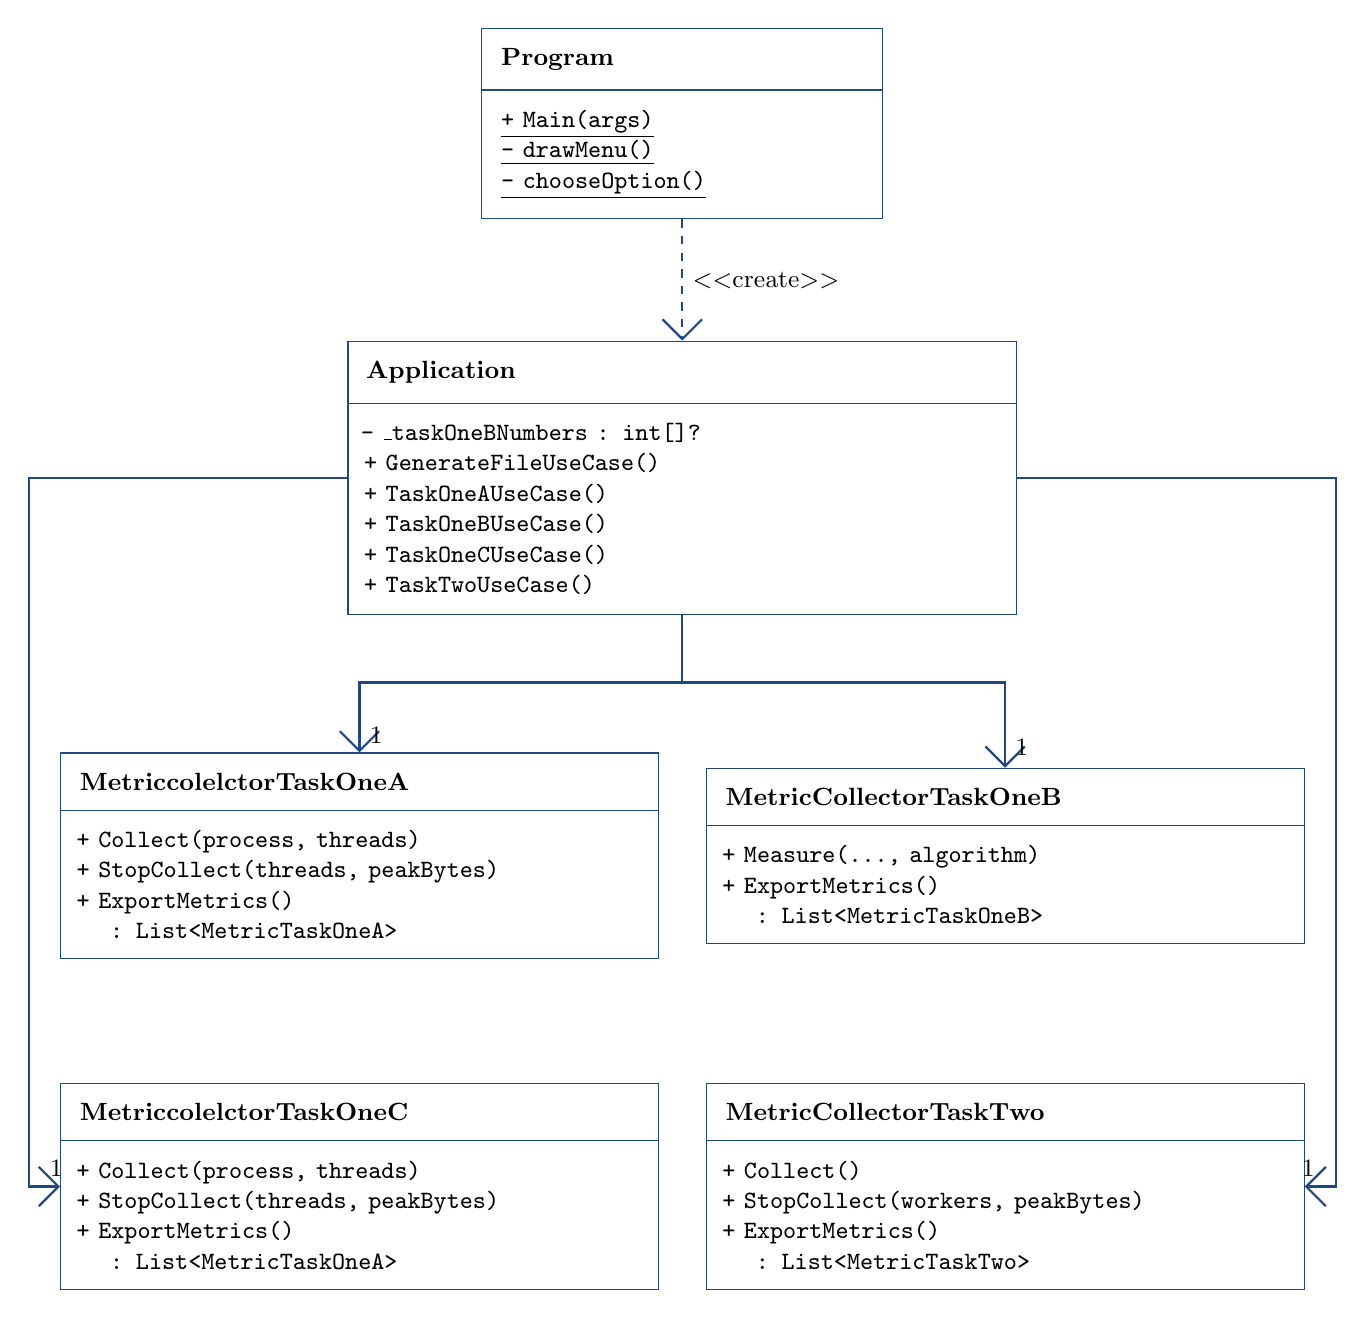
\begin{tikzpicture}[
  umlclass/.style={draw=codeblue,fill=white,rectangle split,rectangle split parts=2,rectangle split part align={center,left},text width=7.1cm,inner sep=7pt,font=\small},
  assoc/.style={-{Straight Barb[length=2.5mm]},line width=.8pt,draw=codeblue},
  dep/.style={assoc,dashed},
  every node/.append style={align=left}]
\node[umlclass,text width=4.6cm] (program) at (0,0) {\textbf{Program}
\nodepart{second}\underline{\texttt{+ Main(args)}}\\\underline{\texttt{- drawMenu()}}\\\underline{\texttt{- chooseOption()}}};
\node[umlclass,text width=8cm] (app) at (0,-4.5) {\textbf{Application}
\nodepart{second}\texttt{- \_taskOneBNumbers : int[]?}\\
\texttt{+ GenerateFileUseCase()}\\
\texttt{+ TaskOneAUseCase()}\\
\texttt{+ TaskOneBUseCase()}\\
\texttt{+ TaskOneCUseCase()}\\
\texttt{+ TaskTwoUseCase()}};
\node[umlclass] (a) at (-4.1,-9.3) {\textbf{MetriccolelctorTaskOneA}
\nodepart{second}\texttt{+ Collect(process, threads)}\\
\texttt{+ StopCollect(threads, peakBytes)}\\
\texttt{+ ExportMetrics()}\\
\texttt{\phantom{+ } : List<MetricTaskOneA>}};
\node[umlclass] (b) at (4.1,-9.3) {\textbf{MetricCollectorTaskOneB}
\nodepart{second}\texttt{+ Measure(..., algorithm)}\\
\texttt{+ ExportMetrics()}\\
\texttt{\phantom{+ } : List<MetricTaskOneB>}};
\node[umlclass] (c) at (-4.1,-13.5) {\textbf{MetriccolelctorTaskOneC}
\nodepart{second}\texttt{+ Collect(process, threads)}\\
\texttt{+ StopCollect(threads, peakBytes)}\\
\texttt{+ ExportMetrics()}\\
\texttt{\phantom{+ } : List<MetricTaskOneA>}};
\node[umlclass] (two) at (4.1,-13.5) {\textbf{MetricCollectorTaskTwo}
\nodepart{second}\texttt{+ Collect()}\\
\texttt{+ StopCollect(workers, peakBytes)}\\
\texttt{+ ExportMetrics()}\\
\texttt{\phantom{+ } : List<MetricTaskTwo>}};
\draw[dep] (program) -- node[right,font=\small]{\textless\textless create\textgreater\textgreater} (app);
\draw[assoc] (app.south) -- (0,-7.1) -| node[pos=.88,right,font=\small]{1} (a.north);
\draw[assoc] (0,-7.1) -| node[pos=.88,right,font=\small]{1} (b.north);
\draw[assoc] (app.west) -- (-8.3,-4.5) |- node[pos=.94,above,font=\small]{1} (c.west);
\draw[assoc] (app.east) -- (8.3,-4.5) |- node[pos=.94,above,font=\small]{1} (two.east);
\end{tikzpicture}
}
\endgroup
\caption{UML class diagram of the controller and metric collectors. Selected members are shown; parameter lists are shortened where marked by dots. A plus sign denotes public access and a minus sign denotes private access. Underlined operations are static.}\label{fig:umlclasses}
\end{figure}

The diagram deliberately preserves the current source names, including \texttt{MetriccolelctorTaskOneA} and \texttt{MetriccolelctorTaskOneC}. The Task 1c collector currently exports \texttt{MetricTaskOneA} records: it reuses their thread/time/memory data shape. Although a separate \texttt{MetricTaskOneC} record is declared in the source, this collector does not use that type. We describe the implementation as it exists rather than introduce a class relationship that is absent from the code.

The records represent measurements, not running tasks. Task 1b records retain the algorithm version, repetition, worker count, time, and all three sign counters. The other active metric records retain a worker/thread count, elapsed time, and peak-memory value; their task programs print sign totals separately. A successful child exit is checked by the menu, while the report's reproduction and validation procedure additionally checks the actual printed counters against the dataset reference.

\section{UML sequence diagram: measure first, visualise later}
Figure~\ref{fig:umlsequence} follows one Task 1a configuration and the later drawing request. The other file-based tasks follow the same launch--wait--collect structure. The diagram's vertical dashed lines are participant lifelines; solid arrows show calls or actions, and dashed arrows show completion or returned information. The narrow rectangles mark periods of execution. The collector is an object in the controller process, while the task and Drawer lifelines represent separate child processes.

\begin{figure}[H]\centering
\begingroup\singlespacing
\resizebox{\textwidth}{!}{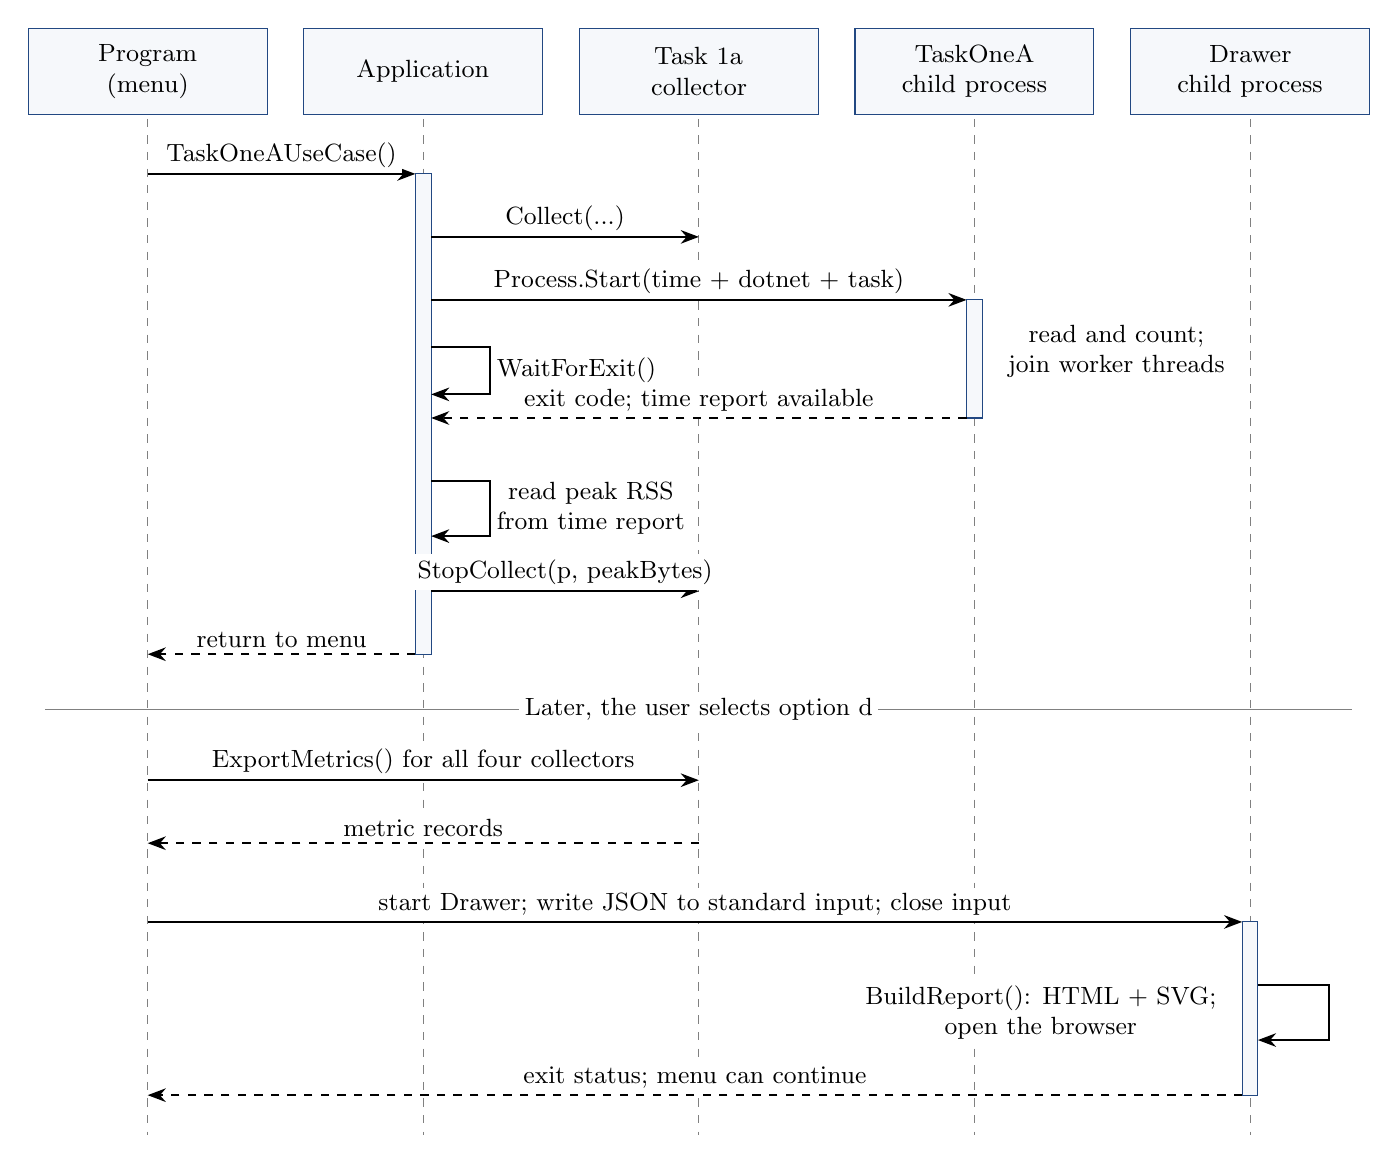
\begin{tikzpicture}[
  head/.style={draw=codeblue,fill=codebg,minimum height=1.1cm,text width=2.8cm,align=center,font=\small},
  call/.style={-{Stealth[length=2.3mm]},line width=.8pt},
  ret/.style={call,dashed},
  msg/.style={font=\small,fill=white,inner sep=2pt,align=center}]
\foreach \name/\x/\label in {menu/0/{Program\\(menu)},app/3.5/{Application},metrics/7/{Task 1a\\collector},task/10.5/{TaskOneA\\child process},drawer/14/{Drawer\\child process}} {
  \node[head] (\name) at (\x,0) {\label};
  \draw[dashed,gray] (\x,-.6) -- (\x,-13.5);
}
\filldraw[draw=codeblue,fill=codebg] (3.4,-1.3) rectangle (3.6,-7.4);
\filldraw[draw=codeblue,fill=codebg] (10.4,-2.9) rectangle (10.6,-4.4);
\filldraw[draw=codeblue,fill=codebg] (13.9,-10.8) rectangle (14.1,-13.0);
\draw[call] (0,-1.3) -- node[msg,above]{TaskOneAUseCase()} (3.4,-1.3);
\draw[call] (3.6,-2.1) -- node[msg,above]{Collect(...)} (7,-2.1);
\draw[call] (3.6,-2.9) -- node[msg,above]{Process.Start(time + dotnet + task)} (10.4,-2.9);
\draw[call] (3.6,-3.5) -- (4.35,-3.5) -- node[msg,right]{WaitForExit()} (4.35,-4.1) -- (3.6,-4.1);
\node[msg,anchor=west] at (10.85,-3.55) {read and count;\\join worker threads};
\draw[ret] (10.4,-4.4) -- node[msg,above]{exit code; time report available} (3.6,-4.4);
\draw[call] (3.6,-5.2) -- (4.35,-5.2) -- node[msg,right]{read peak RSS\\from time report} (4.35,-5.9) -- (3.6,-5.9);
\draw[call] (3.6,-6.6) -- node[msg,above]{StopCollect(p, peakBytes)} (7,-6.6);
\draw[ret] (3.4,-7.4) -- node[msg,above]{return to menu} (0,-7.4);
\draw[gray] (-1.3,-8.1) -- (15.3,-8.1);
\node[msg] at (7,-8.1) {Later, the user selects option d};
\draw[call] (0,-9.0) -- node[msg,above]{ExportMetrics() for all four collectors} (7,-9.0);
\draw[ret] (7,-9.8) -- node[msg,above]{metric records} (0,-9.8);
\draw[call] (0,-10.8) -- node[msg,above]{start Drawer; write JSON to standard input; close input} (13.9,-10.8);
\draw[call] (14.1,-11.6) -- (15,-11.6) -- (15,-12.3) -- (14.1,-12.3);
\node[msg,anchor=east] at (13.65,-11.95) {BuildReport(): HTML + SVG;\\open the browser};
\draw[ret] (13.9,-13.0) -- node[msg,above]{exit status; menu can continue} (0,-13.0);
\end{tikzpicture}
}
\endgroup
\caption{UML sequence diagram for a measured Task 1a run followed by option \texttt{d}. The export step represents all four collectors; the browser itself is outside the displayed participants.}\label{fig:umlsequence}
\end{figure}

First, the collector starts the outer stopwatch. The application then launches \texttt{/usr/bin/time} around the appropriate \texttt{dotnet} task command, waits for completion, checks its exit code, and reads the peak RSS from the time-report file. Finally, it stops collection and saves a metric record. The peak-memory value used by these use cases comes from that report; the presence of a memory-tracking helper elsewhere in a collector does not mean that helper is the active measurement path.

When we later select \texttt{d}, \texttt{Program} exports the four metric lists, serialises their values as JSON, and writes the snapshot to the Drawer's redirected standard input. Closing that input is part of the protocol: \texttt{Drawer.Main} reads until the end of the stream before deserialising. It builds the HTML report, saves it, opens the browser, and returns an exit status. The controller can then display its menu again without waiting for the browser tab to close.

The snapshot is independent of the counting algorithms. Browser checkboxes select which Task 1b runs are drawn and recalculate chart scales; they do not rerun benchmarks or modify the original measured counters. Choosing \texttt{d} again creates a fresh snapshot from the controller's current in-memory records.

\section{How the architecture affects the experiment}
A fresh worker process gives each file-based configuration its own runtime state and peak-RSS high-water mark. It avoids attributing a previous configuration's peak resident memory to the next one. It does not reset the operating system's filesystem cache, which is why the USB reconnect procedure remains necessary.

The controller's cached Task 1b array and the browser live outside a Task 1a/1c/2 child process. Their memory is therefore not part of that child's peak RSS. Conversely, the supplementary Task 1b benchmark loads its array within its own process, so its external process peak includes loading even though its counting stopwatch excludes it. These process boundaries explain the memory scope used throughout the results.

Thread ownership differs inside each algorithm. Task 1a assigns byte ranges before starting workers; Task 1b shares a read-only array but varies ownership of the counters; Task 1c transfers batches through a bounded queue; Task 2 assigns whole-file intervals. We keep those choices inside their task implementations rather than letting the menu manage individual numbers, lines, or queue operations. The following task chapters show the actual source code implementing each choice.

\chapter{Input data, correctness, and measurement method}
\section{Generating and checking the dataset}
We generate \texttt{numbers.txt} with \(N=50\,000\,000\) random integers in the inclusive interval \([-1\,000\,000,1\,000\,000]\), one integer per line. The call to \texttt{Random.Next(minValue, maxValue + 1)} makes the upper limit inclusive. While generating the main file, we also write the same numbers, in the same order, into eight consecutive part files. Each part contains exactly \(6\,250\,000\) lines.

The input used in the measurements occupies \(369\,439\,934\) bytes, approximately \(352.33\) MiB. We checked every line count and computed SHA-256 digests. Concatenating \texttt{numbers1.txt} through \texttt{numbers8.txt} reproduces the main file byte for byte. The manifest in \texttt{data/dataset\_manifest.json} records the exact sizes and hashes. The generator does not store its random seed, so the existing input and its hashes identify this experiment; generating a new input may produce different sign totals.

\begin{lstlisting}[caption={Generating the same ordered data for the main file and the eight parts.}]
int number = random.Next(minValue, maxValue + 1);
mainWriter.WriteLine(number);
partWriter.WriteLine(number);
\end{lstlisting}

For the current dataset, the correct result is
\begin{equation}
N_{-}=24\,996\,544,\qquad N_{+}=25\,003\,426,\qquad N_{0}=30,
\end{equation}
and therefore
\begin{equation}
N_{-}+N_{+}+N_{0}=50\,000\,000.
\end{equation}
A separate validation pass confirmed the reference counters for all seven Task 1a and all seven Task 1c configurations; these validation-pass timings are archived but are not substituted into the earlier performance curves. We require agreement in all three counters, not only in their sum. Equality of a sum alone could hide compensating mistakes. We use the correct per-thread result and the locked implementation as independent implementation checks, and retain validation output from the file-based tasks. The deliberately unsynchronised eight-thread version is expected to fail this check.

\section{What exactly we measure}
For Tasks 1a and 1c, the saved application sessions measure elapsed wall-clock time around launching and waiting for each processing program. File opening, reading, parsing, thread creation, joining, and process/runtime startup are included. We exclude data generation, compilation, chart generation, and report preparation.

In Task 1b, we load the entire file into an \texttt{int[]} before starting the counting stopwatch. The timed region contains only the selected counting method, including its thread creation and final reduction. The raw integer payload alone needs
\begin{equation}
50\,000\,000\times4=200\,000\,000\text{ bytes}\approx190.73\text{ MiB}.
\end{equation}
Object headers, temporary loading allocations, threads, and runtime memory are additional costs. The supplementary Task 1b experiments include one-thread references so that a genuine speed-up relative to one thread can be calculated for each algorithm.

Peak memory is the process-wide maximum resident set size reported by macOS \texttt{/usr/bin/time -l}. On this system it is reported in bytes; we divide by \(2^{20}\) to display MiB. It is resident physical memory, not reserved virtual address space and not just the managed heap. For the supplementary Task 1b measurements, the process peak includes array loading even though loading is excluded from the counting time. Consequently, those memory values describe the whole program's requirement, not an isolated allocation cost of the counting loop.

For Task 2, we measure the complete processing command on the actual USB volume. Before each of the three recorded configurations, we safely eject the drive, physically disconnect it, and reconnect it. Spotlight indexing is disabled and its status is checked after reconnection. We do not read or hash the part-file contents between reconnection and the timed run.

\section{Speed-up and interpretation}
For a fixed algorithm and input, we calculate
\begin{equation}
S(p)=\frac{T(1)}{T(p)},\qquad E(p)=\frac{S(p)}{p}.
\end{equation}
A speed-up above one means that the configuration is faster than its own one-thread reference. A value below one is a slowdown. For example, \(S(p)=3\) means three times faster, not a 300\% reduction in elapsed time. For Task 1b, each version has its own reference; a ratio for the incorrect unsynchronised version is a timing observation only, not a valid speed-up of a correct computation.

We retain two real application snapshots, taken at approximately 15:43 and 16:42. The later snapshot is the primary source for Tasks 1a and 1c; the earlier snapshot provides a limited repeatability check. We do not describe two runs as a statistical confidence interval. The USB results previously shown by the menu have unverified storage/cache provenance and are excluded from the cold-cache USB conclusions. We preserve them in the raw archive rather than silently relabel them.

Background activity, runtime compilation, garbage collection, CPU scheduling, and the filesystem cache can influence timings. The internal-disk experiments did not force a cold cache. We therefore interpret them as measurements of the complete implementation under the recorded conditions, not as isolated SSD throughput or proof of a purely CPU-bound workload.

\chapter{Task 1a: partitioning one file among threads}
\section{Implementation and boundary ownership}
We create \(p\) OS threads for \(p\in\{1,2,4,8,16,32,64\}\). Each thread opens the same file independently and receives a nominal byte interval
\begin{equation}
a_i=\left\lfloor\frac{Li}{p}\right\rfloor,\qquad
b_i=\left\lfloor\frac{L(i+1)}{p}\right\rfloor,
\end{equation}
where \(L\) is the file size in bytes. No single reader loads the whole input first. Each worker uses its own 64 KiB byte buffer and parses integers directly, without allocating a string for every line.

A byte boundary can fall inside an integer. We assign a complete line to the worker whose nominal interval contains the first byte of that line. A worker that starts inside a line skips the remaining bytes of that line. The previous worker is allowed to finish a line that extends beyond its nominal end. This ownership rule prevents both skipping and double counting.

\section{Source code: worker creation, boundaries, and counting}
We include byte-identical snapshots of the submitted task sources, with their original line numbers. Keeping these snapshots inside the LaTeX project allows both a local TeX installation and the editor preview to compile the listings; the supplied synchronisation script verifies their hashes. The first listing creates each worker with its own captured index, computes the byte interval using 64-bit arithmetic, stores any exception in the corresponding error slot, and joins all workers before reading results.

\sourcecode{TaskOneA.cs}{35}{66}{Task 1a: creating workers for separate byte intervals and waiting for completion.}

The complete \texttt{CountPart} method below opens an independent stream for a worker and performs the boundary adjustment. Both possible paths call the same range-counting routine, so a worker whose boundary falls inside a line cannot accidentally bypass the counting logic.

\sourcecode{TaskOneA.cs}{93}{126}{Task 1a: the complete per-worker file-opening and boundary-handling method.}

The counting loop asks \texttt{ReadNumber} for a complete integer only while its current position is inside the nominal interval. The parser advances the shared position reference through the whole current line, including a possible crossing of the nominal end. Each output reference belongs to one worker's counter slot.

\sourcecode{TaskOneA.cs}{128}{153}{Task 1a: classifying complete numbers while their lines belong to the worker.}


The outer counting loop starts another number only while \texttt{position < end}; the integer parser consumes the complete current line. A boundary immediately after a newline needs no adjustment. A boundary on a newline is skipped by the later worker, because the earlier worker owns the line ending there. We join every worker before reading its counters. Worker exceptions are recorded separately and cause the command to fail rather than return a partially successful result.

\section{Measured results}
\input{data/task1a_table}
\resultfigure{task1a.pdf}{Task 1a: elapsed time, speed-up relative to one thread, and peak resident memory. Solid curves are the 16:42 session; dashed curves are the 15:43 repeatability check.}{fig:task1a}

The primary one-thread time is 3876 ms. It decreases to 1505 ms with eight threads, a speed-up of approximately 2.58. The lowest recorded primary time is 1277 ms at 64 threads, approximately 3.04 times faster than one thread. This remains far below ideal linear scaling. In the earlier session, eight threads were fastest at 1475 ms, while 64 threads took 1600 ms. We therefore observe a broad diminishing-returns region rather than a reproducible sharp optimum at one exact thread count.

\section{Answers concerning scaling and memory}
\question{1}{At which thread count does speed-up stop growing, and how does this relate to the CPU?}
The major improvement occurs between one and eight threads, matching the machine's eight logical processors, of which four are performance cores. Beyond roughly 8--16 threads, improvements become much smaller and are inconsistent between sessions. In the primary session, 16, 32, and 64 threads take 1332, 1353, and 1277 ms respectively. The last value is the minimum observed, but the earlier session peaks at eight threads. We cannot honestly claim that the speed-up always stops exactly at eight. We can conclude that adding many more software threads than the eight hardware execution contexts does not provide proportional extra capacity.

\question{2}{Why do 32 and 64 threads not provide large gains? Are they slower?}
They cannot create additional CPU cores. Extra runnable threads add scheduling and context-switching work, compete for caches and memory bandwidth, and can increase file-access and runtime overhead. Reading and parsing also share resources that do not scale with thread count. The serial portions and these overheads limit the benefit of more workers.

The measurements do not support the stronger statement that 32 and 64 threads are always slower. Both are slower than eight threads in the earlier session; 64 is faster than eight in the primary session. Smaller chunks, overlapping waits, and different scheduling/cache conditions may contribute, but identifying the cause would require profiling. We report this variation instead of forcing the observations to match an expected curve.

\question{3}{Does peak memory depend on the number of threads? Why?}
Yes, but the increase is modest here: the primary peak rises from approximately 34.28 MiB at one thread to 38.53 MiB at 64. Every worker adds a buffer, counter/error slots, runtime bookkeeping, and a stack with some resident pages. The explicit buffers alone occupy \(p\times64\) KiB, about 4 MiB at 64 workers. Reserved stack space is not the same as resident memory, so we do not multiply a nominal stack reservation by the thread count and equate it with RSS. This streaming implementation never needs to keep the full 352 MiB text file or 191 MiB integer payload resident in application buffers.

\chapter{Task 1b: shared counters, locking, and local counters}
\section{Three implementations of the same counting operation}
We load the dataset into an integer array before timing, then use eight threads because the runtime reports eight logical processors. The array is read-only during counting, so reading it concurrently does not require a lock. The important difference is where the mutable counters live.

\section{Source code: all three counting methods}
The following listings are the actual methods, including their returned counters. In the first version, the variables are declared outside the worker lambda and are shared captured state. Multiple workers therefore compete to update the same three values.

\sourcecode{TaskOneB.cs}{10}{25}{Task 1b, version 1: unsynchronised shared counters.}

The locked version creates one lock object for the complete invocation. Every worker captures that same object; creating a different lock per worker would not protect shared counters. The classification and counter update are both inside the protected block.

\sourcecode{TaskOneB.cs}{28}{47}{Task 1b, version 2: one shared lock around each classification and increment.}

In the local-counter version, the three variables are declared inside the worker lambda. Only the owning worker changes them. After the helper has joined all threads, the calling thread reduces the result records into one final answer.

\sourcecode{TaskOneB.cs}{50}{78}{Task 1b, version 3: worker-local counting followed by reduction.}

All three methods share the same partitioning mechanism. Its two-argument callback overload delegates to the worker-ID overload shown below. The helper divides the array into half-open index intervals, captures each worker's index, starts the OS threads, and joins them. Consequently, the experimental difference is the counter-update strategy rather than a different partitioning or input-loading scheme.

\sourcecode{TaskOneB.cs}{80}{107}{Task 1b: shared worker-launching helper and disjoint array index ranges.}


The unsynchronised version updates shared captured variables. The locked version uses the same lock object for all workers and acquires it for every number. The local-counter version updates variables owned by one worker, writes one result record per worker, and adds those records after all workers have joined. The \texttt{lock} statement guarantees mutual exclusion for the protected block~\cite{lock}; \texttt{Thread.Join} waits for worker termination before the final aggregation~\cite{join}.

\section{Measurements and correctness}
\input{data/task1b_table}
\resultfigure{task1b_versions.pdf}{Task 1b at eight threads: counting time and retained totals. All three unsynchronised repetitions are shown. A fast but incorrect count is marked as incorrect.}{fig:task1bversions}
\resultfigure{task1b_scaling.pdf}{Supplementary Task 1b measurements at one and eight threads. Each speed-up uses the same version's one-thread baseline. Memory is whole-process peak RSS, including array loading. The unsynchronised eight-thread timing is the mean of three incorrect runs.}{fig:task1bscaling}

\question{4}{Rank the versions by time. Which are correct? Explain each result.}
In the supplementary eight-thread experiment, local counters are fastest at 131.284 ms. The three unsynchronised repetitions take 306.201, 261.485, and 268.229 ms. The locked version is slowest at 1738.592 ms. Thus the observed order is local counters, unsynchronised shared counters, then locked shared counters. The earlier application snapshot gives the same ordering, although its absolute times differ.

Local counters and locking both return the reference totals. The unsynchronised repetitions count only 12\,929\,759, 14\,082\,158, and 12\,389\,943 numbers. They lose approximately 72--75\% of the updates. Their different totals on identical input demonstrate a race condition. The fact that all three retain the 30 zero values does not make the algorithm correct: zero updates are rare and happened not to collide in these runs.

Local counters avoid contention in the hot loop and perform only a small final reduction. Shared counters also cause cache-coherence traffic when cores compete to update the same memory locations, even if no lock is used. A lock makes the update safe but serialises this very small unit of work and repeatedly pays the cost of acquiring and releasing the lock. In this experiment the correct local-counter version is approximately 13.24 times faster than the locked version at eight threads.

The one-thread supplementary measurements make this distinction clearer: local counters take 475.585 ms at one thread and 131.284 ms at eight, giving approximately 3.62 times speed-up. Locking takes 1002.649 ms at one thread and 1738.592 ms at eight, so adding threads slows this version down. A one-thread unsynchronised execution is correct because there is no competing writer; that does not establish correctness once multiple writers are introduced.

\section{How an update is lost}
\begin{table}[H]\centering\small
\caption{A possible interleaving of two increments of the same counter.}\label{tab:race}
\begin{tabularx}{\textwidth}{@{}cXXc@{}}\toprule
Step & Worker A & Worker B & Shared value\\\midrule
1 & Reads 100 & & 100\\
2 & & Reads 100 & 100\\
3 & Computes 101 & & 100\\
4 & & Computes 101 & 100\\
5 & Writes 101 & & 101\\
6 & & Writes 101 & 101\\\bottomrule
\end{tabularx}
\end{table}
Two numbers were processed, but the counter increased only once. The increment is a read--modify--write operation; using a 64-bit counter does not make the whole operation atomic. A lock prevents this interleaving, while thread-local counters remove the competing writes. An atomic increment could also preserve updates, but would still make all workers contend for shared counters and is outside the three required variants.

\chapter{Task 1c: a producer and consumers}
\section{Pipeline, batching, and termination}
We use one dedicated reader and \(p\) worker threads. The reader opens \texttt{numbers.txt}, reads lines, and groups them into batches of 10\,000 strings. A bounded \texttt{BlockingCollection<List<string>>} holds at most 100 batches. Workers repeatedly remove a batch, parse its integers, and update local counters.

\section{Source code: queue lifecycle and both pipeline stages}
The setup below creates the bounded queue and shared cancellation source. The producer signals completion in a \texttt{finally} block, so consumers are not left waiting indefinitely if reading fails. An error is also retained for reporting; cancellation releases blocked queue operations.

\sourcecode{TaskOneC.cs}{30}{57}{Task 1c: queue construction, producer error handling, and guaranteed completion signalling.}

The complete producer method forms batches of \texttt{BatchSize = 10000} lines. The queue capacity is \texttt{QueueCapacity = 100} batches. Publishing a full batch transfers its list to consumers; the producer then allocates a new list, so it does not keep appending to a list already being processed elsewhere.

\sourcecode{TaskOneC.cs}{128}{153}{Task 1c: reading lines, publishing full batches, and handling the final partial batch.}

The complete consumer method removes batches through consuming enumeration, validates every integer, and updates its own output slots. It naturally finishes when no more batches can arrive and the queue has been drained. The enclosing worker catches errors and requests shared cancellation, following the same failure policy as the producer.

\sourcecode{TaskOneC.cs}{155}{189}{Task 1c: the complete consumer parsing and counting loop.}

Once all participants have been constructed, we start the reader and consumers, join the reader, and then join every consumer. Waiting for the producer alone would be insufficient because queued batches could still be in progress.

\sourcecode{TaskOneC.cs}{85}{95}{Task 1c: starting the pipeline and joining both producer and consumers.}


This queue provides both thread-safe transfer and backpressure: an empty queue makes consumers wait, and a full queue makes the producer wait~\cite{blocking}. There is no busy loop checking for available work. Completion is different from cancellation: on normal completion, queued batches are still processed; on an error, the shared cancellation token releases blocked operations so that the program can report failure rather than deadlock. The producer also publishes the final partial batch if the input size is not a multiple of 10\,000.

\resultfigure{pipeline.pdf}{Task 1c separates the sequential line reader from parallel integer parsing. The queue bounds waiting batches; additional batches can also be held by the producer and active workers.}{fig:pipeline}

\section{Measured results and comparison}
\input{data/task1c_table}
\resultfigure{task1c.pdf}{Task 1c: time, speed-up relative to one worker, and peak resident memory in the two real saved sessions. The horizontal reference in the speed-up panel represents the one-worker time.}{fig:task1c}

\question{5}{How does Task 1c compare with Task 1a, and when does it stop getting faster?}
In the primary session, Task 1c takes 1952 ms with one worker, versus 3876 ms for Task 1a with one thread. Task 1c includes a separate producer, so ``one worker'' already means two active processing threads, in addition to the coordinating main thread. This is not a comparison of two single-threaded programs. Overlapping reading/line extraction with parsing can help, and the implementations also use different parsing and buffering paths.

Task 1c reaches its best primary time at two workers: 1853 ms, only about 1.05 times faster than its one-worker configuration. At four workers Task 1a is already faster: 1834 ms versus 1984 ms. With eight workers the gap grows to 1505 ms versus 2248 ms. Task 1c reaches 3413 ms at 64 workers, slower than its own one-worker configuration.

The sequential producer must read every line and allocate strings. Every batch also crosses a synchronised queue. Additional consumers cannot accelerate the producer and eventually add contention, scheduling work, and allocation/garbage-collection pressure. Task 1a instead lets workers read independent byte ranges and parse directly into local counters. In these measurements, Task 1c stops providing a useful improvement after about 1--2 workers; the earlier session is already fastest at one worker. The best Task 1c primary configuration is not the best configuration overall.

Peak memory is not monotonic: the primary session uses approximately 131.56 MiB at one worker, falls to 50.16 MiB at four, and rises to 137.05 MiB at 64. With few consumers the queue can accumulate strings; adding consumers can drain it faster. At large worker counts, active batches, thread resources, and runtime overhead grow. A bounded queue limits queued items, but does not force identical occupancy or identical RSS in every run.

\question{6}{What changes with one-line batches or an unbounded queue?}
The current dataset produces exactly 5000 batches of 10\,000 lines. One-line batches would require 50 million queue transfers, 10\,000 times as many. That increases synchronisation, wake-up, bookkeeping, and small-allocation costs relative to the very cheap operation of classifying one integer. Smaller batches can improve balancing for expensive or irregular work, but a batch of one is a poor trade-off for this workload.

The present queue can hold at most one million waiting lines. This is not the total number of live lines: the producer may be building a batch, and each worker may hold another batch. With an unbounded queue, a fast producer can run far ahead and retain a large fraction of the 50 million strings, consuming far more memory than their compact integer representation. Garbage collection, memory pressure, and possibly swapping can then reduce throughput. Bounding the queue makes the producer wait and keeps the amount of queued work under control; it does not by itself remove all other sources of memory growth.

\chapter{Task 2: eight files on the USB flash drive}
\section{Implementation and cold-cache procedure}
We place the eight ordered part files on \texttt{/Volumes/ESD-USB}. A file is the unit of work. Each worker reads a whole assigned file with \texttt{File.ReadAllBytes}, parses the returned byte buffer, updates local counters, and proceeds to its next file. The library method returns a byte array containing the complete file~\cite{readallbytes}. One application-level read call does not imply that the operating system performs exactly one physical USB request.

\section{Source code: file assignment, buffering, and parsing}
The actual worker-creation loop assigns a half-open interval of file indices to each thread. The captured \texttt{workerIndex} chooses both the interval and the worker's output/error slots. All workers are joined before the caller checks errors and combines the counters.

\sourcecode{TaskTwo.cs}{45}{74}{Task 2: balanced file assignment, worker startup, and completion.}

The complete \texttt{CountFiles} method reads one assigned file at a time into one byte array. It does not construct a list of lines. Each buffer is parsed before the worker advances to its next file.

\sourcecode{TaskTwo.cs}{101}{118}{Task 2: whole-file byte-buffer reading for each assigned file.}

The parser first skips separators (the preceding part of \texttt{CountNumbers}), then performs the sign, digit, and classification logic shown below. \texttt{checked} prevents silently wrapping an out-of-range value. The remainder of the method rejects non-separator characters after an integer, so malformed input is reported rather than counted as a successful partial read.

\sourcecode{TaskTwo.cs}{143}{178}{Task 2: actual sign parsing, checked digit accumulation, and classification inside CountNumbers.}


With one thread, the worker processes eight files sequentially; with two, each handles four files; with four, each handles two. We use only the required 1, 2, and 4 threads for the cold-cache experiment. Using more than eight threads would leave some workers without an assigned file because there are only eight independent work units.

We disabled Spotlight indexing on the volume. Before each measurement, we safely ejected the device, unplugged it, and reconnected it. We checked that indexing remained disabled, then immediately ran the relevant configuration without previewing or reading the input files. All three commands use the explicit absolute USB directory. We corrected the previous relative path \texttt{Volumes/ESD-USB}; without its leading slash it referred to a different location relative to the current working directory.

\section{Measured results}
\input{data/task2_table}
\resultfigure{task2.pdf}{Task 2: actual USB reads after a separate physical reconnect for every configuration. Speed-up uses the cold one-thread USB time. Peak memory includes complete-file byte buffers and runtime allocations.}{fig:task2}

Every cold-cache run returns the same three reference counters and a total of 50 million. The input volume and individual file contents are the same workload as in Task 1, but buffering and parsing implementations differ; this matters when comparing absolute times.

\section{Answers about storage and concurrency}
\question{1}{How does one USB thread compare with one internal-disk thread? Is the USB work CPU-bound or I/O-bound?}
Task 1a on one thread takes 3876 ms in the primary internal-disk session. The cold USB run takes \USBOneMs{} ms, a ratio of approximately \USBvsSSD{}. The USB command's application throughput is about \USBOneMBs{} MB/s, calculated from the full input byte size and elapsed time. This is application throughput, including parsing and startup, not an isolated benchmark of the USB link.

The one-thread USB process uses 1.95 s of user CPU time and 0.12 s of system CPU time during 4.67 s of measured real time. Thus approximately 2.07 s of CPU time accounts for only about 44\% of the elapsed time. This indicates a substantial non-CPU component, consistent with waiting for cold external-storage reads. It does not mean that every remaining millisecond can be attributed exclusively to the flash hardware: scheduling and runtime behaviour also contribute.

We classify this cold USB workload as storage-sensitive, with a substantial I/O-wait component, rather than purely CPU-bound. We also avoid claiming that the whole difference from Task 1a is caused by the drive: Task 1a streams 64 KiB buffers, whereas Task 2 allocates whole-file buffers and uses a different parser. A stricter isolation of device cost would run the same Task 2 algorithm on both devices under matched cache conditions.

\question{2}{Do more USB threads help? Why is this different from a server waiting on the network?}
The measured times are \USBOneMs{}, \USBTwoMs{}, and \USBFourMs{} ms for one, two, and four threads, giving speed-ups of \USBSpeedTwo{} and \USBSpeedFour{} for two and four threads. \USBScalingInterpretation{} The four-thread run is only about 0.4\% slower than the two-thread run. With one run per USB configuration, we treat this as a plateau rather than evidence of a statistically established regression.

All workers still share one flash device and its controller. Additional threads may overlap parsing with reading and may keep outstanding work available, but they do not multiply the drive's total bandwidth. Concurrent reads can also interfere with otherwise sequential access. The useful concurrency level therefore depends on the drive and workload, not simply on the fact that the operation involves I/O.

For a network server, different requests can be waiting for independent remote services or clients. While one request waits for a response, another may use the CPU or a different connection. Concurrency can hide these separate latency intervals before a shared resource becomes saturated. A single USB drive presents a much more direct shared-throughput limit. The lecture's general lesson remains valid, but it does not guarantee linear speed-up for concurrent reads from one physical device.

Peak RSS also increases when several complete input buffers are live together. Each file is about 44 MiB. Garbage collection may retain arrays from previously processed files until a collection occurs, so peak memory is not guaranteed to be exactly one file size per worker. The measured RSS includes those arrays, runtime memory, thread resources, and allocation history.

\clearpage
\chapter{Answers to all control questions}
\question{1}{What is the difference between a physical core and a logical processor? Where does it appear in our charts?}
A physical core is a hardware execution core. A logical processor is an execution context exposed by the processor and OS to the scheduler. On a processor with simultaneous multithreading, several logical processors may share one physical core's execution resources. On our Apple M3, macOS exposes eight logical processors for eight physical cores: four performance and four efficiency cores. We therefore do not have an additional hardware doubling beyond eight.

In Task 1a, the substantial early gains and much smaller, variable gains beyond 8--16 software threads are consistent with this finite CPU capacity. In Task 1c, the reader and queue limit scaling long before all hardware contexts become useful. The charts show why core count is an upper-resource constraint rather than a guarantee that every algorithm reaches its optimum at exactly that count.

\question{2}{How do we ensure that no line is counted twice or skipped between two file parts?}
We define ownership by the line's starting byte. A worker begins at its nominal boundary only if that boundary follows a newline. Otherwise it advances to the next complete line. At the other end, it finishes any line whose first byte it already owns, even when that line crosses the nominal boundary. The next worker skips that same partial line. These two rules fit together: the earlier worker owns the crossing line, and the later worker owns the next line. We also check all three sign counts against the common reference and verify that the ordered part files reproduce the main file.

\question{3}{How do unsynchronised shared counters lose updates, step by step?}
First, one worker reads a counter value. Before it writes back, another worker reads the same old value. Each computes the old value plus one. Both then write the same new value, so one increment overwrites the effect of the other. Table~\ref{tab:race} shows a concrete interleaving from 100 to 101 instead of 102. This remains possible even when individual reads and writes of the counter fit in a machine word, because the whole increment contains multiple operations. The differing incorrect totals in our three repetitions demonstrate the practical consequence.

\question{4}{Why are per-thread counters faster than shared counters protected by a lock?}
Each worker can increment its own variables without acquiring a shared lock on every number. The hot loops run independently, and the final reduction costs only a few additions per worker after joining. A shared lock serialises the protected block and can force waiting, ownership transfers, and scheduling work. Even an extremely short critical section becomes expensive when we enter it 50 million times. Our eight-thread local-counter measurement is 131.284 ms, versus 1738.592 ms for locking, while both produce the same correct totals.

\question{5}{What does I/O-bound mean for a USB drive and for a network server? Why can their response to concurrency differ?}
I/O-bound means that waiting for input/output, rather than available CPU computation alone, limits progress. For our cold USB run, the process spends much less CPU time than real elapsed time and all reads share the same device. Several threads cannot create additional flash bandwidth. For a server, waiting can concern many independent requests, remote computers, or network round trips, so concurrency can use otherwise idle CPU time while those waits overlap.

The statement that concurrency helps only the network case is a useful simplification, not a universal rule. USB concurrency can also help when it overlaps parsing with reading, hides device latency, or improves the controller's utilisation; our actual speed-up must be read from the measured curve. It eventually encounters a shared device limit. A network service can likewise stop benefiting once its CPU, connection limits, or network bandwidth are saturated.

\question{6}{How does static partitioning differ from taking work from a queue? When is each preferable?}
Static partitioning assigns each worker a fixed range before processing starts. Tasks 1a and 2 use this approach. It has little coordination overhead and is effective when work units are sufficiently uniform. Its weakness is imbalance: a worker that finishes early cannot automatically take a portion of a slower worker's assignment. Equal bytes also do not necessarily mean exactly equal parsing time.

Queue-based scheduling assigns the next available unit to whichever worker finishes and requests more work. Task 1c can therefore balance consumers dynamically when batch costs differ. It also adds a producer, queue operations, synchronisation, and a need for termination/backpressure rules. We prefer static partitioning for cheap, regular work where independence is easy to arrange, and a bounded queue for streaming pipelines or work with variable processing costs. Our measurements show that dynamic scheduling is not automatically faster when the producer itself is the bottleneck.

\chapter{Build, run, and inspect the implementation}
\section{Source organisation and command-line entry point}
The submitted C\# sources are in \texttt{code/}. \texttt{TaskOneA.cs}, \texttt{TaskOneB.cs}, \texttt{TaskOneC.cs}, and \texttt{TaskTwo.cs} implement the algorithms; \texttt{Program.cs} provides the interactive menu and metric collectors; \texttt{Drawer.cs} builds the browser dashboard. We provide \texttt{documentation/reproduce/lab1.sh} as one command-line entry point for selecting tasks and configurations without navigating the menu. The implementation remains organised as separate file-based C\# modules, launched by the entry point.

From the laboratory directory, we build before measuring:
\begin{lstlisting}[language=bash,caption={Preparing the file-based executables.}]
cd Lab1.Concurrency-in-practice
bash documentation/reproduce/lab1.sh build
\end{lstlisting}

The following examples select every task explicitly. The second argument is the number of processing threads or consumers. For Task 1b, the version and repetition label are additional arguments; loading the integer array remains outside the internal stopwatch.
\begin{lstlisting}[language=bash,caption={Examples for all four tasks.}]
bash documentation/reproduce/lab1.sh task1a 8
bash documentation/reproduce/lab1.sh task1b 8 Unsynchronized 1
bash documentation/reproduce/lab1.sh task1b 8 Unsynchronized 2
bash documentation/reproduce/lab1.sh task1b 8 Unsynchronized 3
bash documentation/reproduce/lab1.sh task1b 8 Locked 1
bash documentation/reproduce/lab1.sh task1b 8 LocalCounters 1
bash documentation/reproduce/lab1.sh task1c 2
bash documentation/reproduce/lab1.sh task2 1 /Volumes/ESD-USB
\end{lstlisting}

For Tasks 1a and 1c, we repeat the command with 1, 2, 4, 8, 16, 32, and 64 workers. For Task 1b, eight workers satisfy the required logical-processor setting; one worker is an additional baseline used only to calculate scaling. For Task 2, we run 1, 2, and 4 separately, with a physical reconnect before each, rather than putting all configurations in an uninterrupted loop.

If the existing input is absent, menu option \texttt{g} generates the main file and the eight parts. Re-generating input changes the experiment, so we keep the original files for comparison with the recorded hashes. The USB must contain the eight part files before beginning cold-cache measurements; copying and checking them belongs before the eject/reconnect sequence.

\section{Measuring a processing command on macOS}
\begin{lstlisting}[language=bash,caption={An example of whole-process timing and peak-memory capture.}]
cd code
/usr/bin/time -l -o task1a-8.time.txt \
  dotnet artifacts/TaskOneA/TaskOneA.dll 8
\end{lstlisting}
The \texttt{real} value is wall-clock time; \texttt{user} and \texttt{sys} record CPU time. We retain the maximum resident set size and the printed sign totals. For Task 1b, we use the benchmark's internal \texttt{ELAPSED\_MS} value for counting time and the external process peak for memory. Timing a complete \texttt{dotnet run} compilation command would add build overhead and would not reproduce that counting metric.

\section{USB preparation and access}
\begin{lstlisting}[language=bash,caption={Checking and preparing the USB volume.}]
diskutil list external physical
ls /Volumes
diskutil info /Volumes/ESD-USB
mdutil -i off /Volumes/ESD-USB
mdutil -s /Volumes/ESD-USB
cd ~
diskutil eject /Volumes/ESD-USB
# Physically unplug and reconnect, then measure one configuration.
\end{lstlisting}
The absolute path begins with \texttt{/Volumes}. A terminal whose working directory is inside the USB volume can prevent safe ejection; changing to the home directory releases that reference. We do not force-unmount the drive. If the operating system requires administrative privileges for indexing control, that preparation is performed with the appropriate local authorisation before the timed experiment.

\section{Dashboard and evidence}
Launching \texttt{dotnet run --file Program.cs} from \texttt{code/} opens the original menu. After collecting metrics, option \texttt{d} passes all four metric sets to \texttt{Drawer.cs}, which generates an offline HTML report and opens it in a browser. Task 1b has individual run checkboxes. Unchecking \texttt{Locked} removes it from both graphs and recalculates their scales, making the smaller timing differences visible. The exact-value table retains every original measurement.

The report uses vector plots and searchable source listings for readable results and code. We retain the original real dashboard snapshots, CSV/JSON measurements, dataset manifest, and per-run timing/output logs in \texttt{report/data/}. The accompanying scripts reproduce the figures and processing commands.

\clearpage
\chapter{Conclusions}
We found that the organisation of the work matters at least as much as the number of threads. Task 1a gains substantially from partitioning a single file across workers: the primary time decreases from 3876 to 1277 ms, but returns beyond 8--16 threads are small and unstable between sessions. We interpret this as CPU-sensitive parsing combined with shared memory, I/O, scheduling, and runtime costs; without matched cold-cache tests or profiling, we do not describe the internal-disk task as purely CPU-bound.

We classify Task 1b as an in-memory CPU/memory-bound counting workload: input loading is outside the timed region, and the counting loops perform no file I/O. It is our clearest CPU-side comparison, although memory bandwidth and shared-cache traffic can still limit scaling. Per-thread counters are both correct and fastest in our eight-thread measurements. The locked version is correct but much slower because it serialises millions of small updates. The unsynchronised version returns different incorrect totals on the same input. Its elapsed time therefore cannot be used as evidence of a successful correct optimisation.

Task 1c demonstrates a different scaling limit. Its bounded queue prevents unlimited producer lead, but the single reader, string allocation, and queue transfers restrict throughput. The primary optimum occurs at two consumers, and 64 consumers are slower than one. Memory depends on queue occupancy and active batches as well as thread count, which explains why its peak RSS is not monotonic.

The cold USB experiment introduces a substantial storage-wait component: one thread needs \USBOneMs{} ms for the same dataset, compared with 3876 ms in the primary one-thread Task 1a session. The USB run uses only about 2.07 s of CPU time during 4.67 s of real time. Additional workers achieve the measured speed-ups of \USBSpeedTwo{} and \USBSpeedFour{}, while continuing to share one flash device. We therefore distinguish latency overlap from multiplying storage bandwidth, and we keep the USB conclusions separate from earlier measurements with unverified cache provenance.

Our practical recommendation for this workload is to use independent counters and a small, measured degree of concurrency, to verify all counters before interpreting timings, and to keep cache conditions explicit. The best worker count is an experimental result, not a value that can be inferred from core count alone.

\clearpage
\phantomsection
\addcontentsline{toc}{chapter}{Bibliography}
\begin{thebibliography}{9}
\singlespacing\normalsize\raggedright
\urlstyle{same}
\bibitem{lab} Network Programming. \emph{Laboratory Work 1: Concurrency in Practice}. Course handout supplied with this laboratory, four pages. Requirements, task questions, control questions, and grading criteria.
\bibitem{apple} Apple. \emph{MacBook Air (15-inch, M3, 2024): Technical Specifications}. \url{https://support.apple.com/en-us/118552}. Accessed 25 October 2026.
\bibitem{blocking} Microsoft. \emph{BlockingCollection Overview}. .NET documentation. \url{https://learn.microsoft.com/en-us/dotnet/standard/collections/thread-safe/blockingcollection-overview}. Accessed 25 October 2026.
\bibitem{lock} Microsoft. \emph{C\# Language Specification: Statements, Section 13.13, the lock statement}. \url{https://learn.microsoft.com/en-us/dotnet/csharp/language-reference/language-specification/statements}. Accessed 25 October 2026.
\bibitem{join} Microsoft. \emph{Thread.Join Method}. .NET API documentation. \url{https://learn.microsoft.com/en-us/dotnet/api/system.threading.thread.join}. Accessed 25 October 2026.
\bibitem{readallbytes} Microsoft. \emph{File.ReadAllBytes Method}. .NET API documentation. \url{https://learn.microsoft.com/en-us/dotnet/api/system.io.file.readallbytes}. Accessed 25 October 2026.
\end{thebibliography}

\end{document}
